\gdef\sfill{white}
\gdef\Afill{white}
\gdef\Bfill{white}
\gdef\Cfill{white}
\gdef\Dfill{white}
\gdef\Efill{white}
\gdef\Ffill{white}
\gdef\Gfill{white}

\gdef\sdesc{s}
\gdef\Adesc{A}
\gdef\Bdesc{B}
\gdef\Cdesc{C}
\gdef\Ddesc{D}
\gdef\Edesc{E}
\gdef\Fdesc{F}
\gdef\Gdesc{G}
\gdef\Gfill{green}
\gdef\Gdesc{G[8/9]}
\gdef\Ffill{green}
\gdef\Fdesc{F[7/10]}
\gdef\Cfill{green}
\gdef\Cdesc{C[6/11]}
\gdef\Efill{green}
\gdef\Edesc{E[5/12]}
\gdef\Bfill{green}
\gdef\Bdesc{B[4/13]}
\gdef\Dfill{green}
\gdef\Ddesc{D[3/14]}
\gdef\Afill{green}
\gdef\Adesc{A[2/15]}
\gdef\sfill{green}
\gdef\sdesc{s[1/16]}
\subsection*{6.1.5 SCC}
\subsubsection*{Schritt 1: Aufruf von DFS(G) zur Berechnung der Endzeiten $f[v]$}
\gdef\ndist{2.5cm}
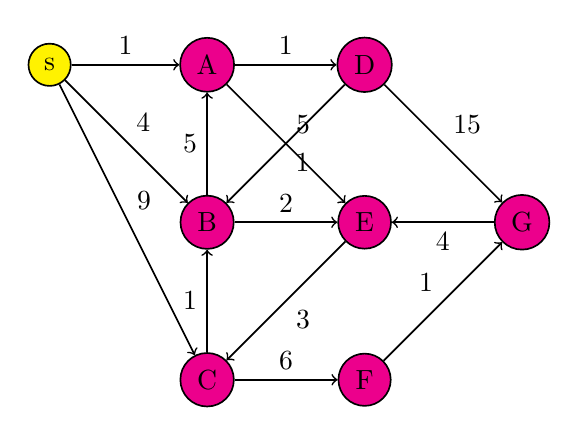
\begin{tikzpicture}[->, semithick,auto, node distance=2cm]


\node[draw, circle, fill=\sfill] (s) at (0,0) {s};
\node[draw, circle, fill=\Afill] (A) [right of=s] {A};
\node[draw, circle, fill=\Bfill] (B) [below of=A] {B};
\node[draw, circle, fill=\Cfill] (C) [below of=B] {C};
\node[draw, circle, fill=\Dfill] (D) [right of=A] {D};
\node[draw, circle, fill=\Efill] (E) [below of=D] {E};
\node[draw, circle, fill=\Ffill] (F) [below of=E] {F};
\node[draw, circle, fill=\Gfill] (G) [right of=E] {G};

\path 	(s) 	edge node {1} (A)
		edge node {4} (B)
		edge node {9} (C)
	(A) 	edge node {1} (D)
		edge node {5} (E)
	(B) 	edge node {5} (A)
		edge node {2} (E)
	(C) 	edge node {1} (B)
		edge node {6} (F)
	(D) 	edge node {1} (B)
		edge node {15} (G)
	(E) 	edge node {3} (C)
	(F) 	edge node {1} (G)
	(G) 	edge node {4} (E)
	;

\end{tikzpicture}



\subsubsection*{Schritt 2: Berechne $G^T$ (transponierter Graph)}
\begin{tikzpicture}[->, semithick,auto, node distance=2.5cm]


\node[draw, circle, fill=\sfill] (s) at (0,0) {\sdesc};
\node[draw, circle, fill=\Afill] (A) [right of=s] {\Adesc};
\node[draw, circle, fill=\Bfill] (B) [below of=A] {\Bdesc};
\node[draw, circle, fill=\Cfill] (C) [below of=B] {\Cdesc};
\node[draw, circle, fill=\Dfill] (D) [right of=A] {\Ddesc};
\node[draw, circle, fill=\Efill] (E) [below of=D] {\Edesc};
\node[draw, circle, fill=\Ffill] (F) [below of=E] {\Fdesc};
\node[draw, circle, fill=\Gfill] (G) [right of=E] {\Gdesc};

\path[draw=\sAcolor]	(A) 	edge node {1} (s);
\path[draw=\sBcolor] 	(B)	edge node {4} (s);
\path[draw=\sCcolor] 	(C)	edge node {9} (s);
\path[draw=\ADcolor] 	(D) 	edge node {1} (A);
\path[draw=\AEcolor] 	(E)	edge node {5} (A);
\path[draw=\BAcolor] 	(A) 	edge node {5} (B);
\path[draw=\BEcolor] 	(E)	edge node {2} (B);
\path[draw=\CBcolor] 	(B) 	edge node {1} (C);
\path[draw=\CFcolor] 	(F)	edge node {6} (C);
\path[draw=\DBcolor] 	(B) 	edge node {1} (D);
\path[draw=\DGcolor] 	(G)	edge node {15} (D);
\path[draw=\ECcolor] 	(C) 	edge node {3} (E);
\path[draw=\FGcolor] 	(G) 	edge node {1} (F);
\path[draw=\GEcolor] 	(E) 	edge node {4} (G);

\end{tikzpicture}

\subsubsection*{Schritt 3: Aufruf von DFS($G^T$)}
Im folgenden sind die Werte in runden Klammern die Zeiten beim Aufruf von DFS($G^T$). Hierbei werden die vorherigen Zeiten pro Baum ersetzt.\\
Wir beginnen die Tiefensuche beim Knoten $v$ mit dem größten Wert für $f[v]$(DFS(G)) und betrachten die Knoten in Reihenfolge fallender $f[v]$.
Die Bäume sind farblich hervorgehoben.

\gdef\sdesc{s(1/2)}
\gdef\sfill{yellow}
\begin{tikzpicture}[->, semithick,auto, node distance=2.5cm]


\node[draw, circle, fill=\sfill] (s) at (0,0) {\sdesc};
\node[draw, circle, fill=\Afill] (A) [right of=s] {\Adesc};
\node[draw, circle, fill=\Bfill] (B) [below of=A] {\Bdesc};
\node[draw, circle, fill=\Cfill] (C) [below of=B] {\Cdesc};
\node[draw, circle, fill=\Dfill] (D) [right of=A] {\Ddesc};
\node[draw, circle, fill=\Efill] (E) [below of=D] {\Edesc};
\node[draw, circle, fill=\Ffill] (F) [below of=E] {\Fdesc};
\node[draw, circle, fill=\Gfill] (G) [right of=E] {\Gdesc};

\path[draw=\sAcolor]	(A) 	edge node {1} (s);
\path[draw=\sBcolor] 	(B)	edge node {4} (s);
\path[draw=\sCcolor] 	(C)	edge node {9} (s);
\path[draw=\ADcolor] 	(D) 	edge node {1} (A);
\path[draw=\AEcolor] 	(E)	edge node {5} (A);
\path[draw=\BAcolor] 	(A) 	edge node {5} (B);
\path[draw=\BEcolor] 	(E)	edge node {2} (B);
\path[draw=\CBcolor] 	(B) 	edge node {1} (C);
\path[draw=\CFcolor] 	(F)	edge node {6} (C);
\path[draw=\DBcolor] 	(B) 	edge node {1} (D);
\path[draw=\DGcolor] 	(G)	edge node {15} (D);
\path[draw=\ECcolor] 	(C) 	edge node {3} (E);
\path[draw=\FGcolor] 	(G) 	edge node {1} (F);
\path[draw=\GEcolor] 	(E) 	edge node {4} (G);

\end{tikzpicture}

\gdef\Adesc{A(3/16)}
\gdef\Afill{magenta}
\gdef\Bdesc{B(4/15)}
\gdef\Bfill{magenta}
\gdef\Cdesc{C(5/14)}
\gdef\Cfill{magenta}
\gdef\Edesc{E(6/13)}
\gdef\Efill{magenta}
\gdef\Gdesc{G(7/12)}
\gdef\Gfill{magenta}
\gdef\Ddesc{D(8/9)}
\gdef\Dfill{magenta}
\gdef\Fdesc{F(10/11)}
\gdef\Ffill{magenta}
\begin{tikzpicture}[->, semithick,auto, node distance=2.5cm]


\node[draw, circle, fill=\sfill] (s) at (0,0) {\sdesc};
\node[draw, circle, fill=\Afill] (A) [right of=s] {\Adesc};
\node[draw, circle, fill=\Bfill] (B) [below of=A] {\Bdesc};
\node[draw, circle, fill=\Cfill] (C) [below of=B] {\Cdesc};
\node[draw, circle, fill=\Dfill] (D) [right of=A] {\Ddesc};
\node[draw, circle, fill=\Efill] (E) [below of=D] {\Edesc};
\node[draw, circle, fill=\Ffill] (F) [below of=E] {\Fdesc};
\node[draw, circle, fill=\Gfill] (G) [right of=E] {\Gdesc};

\path[draw=\sAcolor]	(A) 	edge node {1} (s);
\path[draw=\sBcolor] 	(B)	edge node {4} (s);
\path[draw=\sCcolor] 	(C)	edge node {9} (s);
\path[draw=\ADcolor] 	(D) 	edge node {1} (A);
\path[draw=\AEcolor] 	(E)	edge node {5} (A);
\path[draw=\BAcolor] 	(A) 	edge node {5} (B);
\path[draw=\BEcolor] 	(E)	edge node {2} (B);
\path[draw=\CBcolor] 	(B) 	edge node {1} (C);
\path[draw=\CFcolor] 	(F)	edge node {6} (C);
\path[draw=\DBcolor] 	(B) 	edge node {1} (D);
\path[draw=\DGcolor] 	(G)	edge node {15} (D);
\path[draw=\ECcolor] 	(C) 	edge node {3} (E);
\path[draw=\FGcolor] 	(G) 	edge node {1} (F);
\path[draw=\GEcolor] 	(E) 	edge node {4} (G);

\end{tikzpicture}

\subsubsection*{Schritt 4: Strenge Zusammenhangskomponenten}
Die einzelnen Bäume in der obigen Grafik bilden die strengen Zusammenhangskomponenten unserer Graphen $G$, sowie $G^T$.